\documentclass[xcolor=table,xcdraw,aspectratio=169]{beamer}
\usepackage{beamerthemesplit}
\usepackage{wrapfig}
\usetheme{SPbGU}
\usepackage{pdfpages}
\usepackage{amsmath}
\usepackage{cmap} 
\usepackage[T2A]{fontenc} 
\usepackage[utf8]{inputenc}
\usepackage[english,russian]{babel}
\usepackage{indentfirst}
\usepackage{amsmath}
\usepackage{multirow}
\usepackage[noend]{algpseudocode}
\usepackage{algorithm}
\usepackage{algorithmicx}
\usepackage{csvsimple}
\usepackage{booktabs}
\usepackage{adjustbox}
% \usetikzlibrary{shapes,arrows}
\usepackage{fancyvrb}
\usepackage{algpseudocode}
\usepackage{algorithm}
\usepackage{algorithmicx}
\usepackage{verbatim}
\usepackage{mathtools}
\usepackage{multirow}
\usepackage{subcaption}

\usepackage{fontawesome}
\usepackage{array}

\usepackage{tikz}
\usetikzlibrary{automata,positioning}
\usepackage{svg}
% \usepackage[table,xcdraw]{xcolor}

\usepackage[most]{tcolorbox}

\newtheorem{rutheorem}{Теорема}
\newtheorem{ruproof}{Доказательство}
\newtheorem{rudefinition}{Определение}
\newtheorem{rulemma}{Лемма}
\beamertemplatenavigationsymbolsempty

\title[Модернизация CFPQ\_Data]{Модернизация набора данных \textsc{CFPQ\_Data}}
% То, что в квадратных скобках, отображается в левом нижнем углу. 
\institute[СПбГУ]{
Санкт-Петербургский государственный университет \\
Кафедра системного программирования }

% То, что в квадратных скобках, отображается в левом нижнем углу.
\author[Вадим Абзалов]{Вадим Игоревич Абзалов, 18.Б11-мм \\
  % У научного руководителя должна быть указана научная степень
  \and  
    {\bfseries Научный руководитель:} к.\,ф.-м.\,н., доцент кафедры информатики СПбГУ С.\,В. Григорьев}

\date{\today}

\definecolor{orange}{RGB}{179,36,31}

\begin{document}
{
% Лого университета или организации, отображается в шапке титульного листа
\begin{frame}
  \begin{center}
  {
\includegraphics[width=1.5cm]{img/SPbGU_Logo.png}}
  \end{center}
  \titlepage
\end{frame}
}

\section{Introduction}

Scalable high-performance graph analysis is an actual challenge.
There is a big number of ways to attack this challenge~\cite{Coimbra2021} and the first promising idea is to utilize general-purpose graphic processing units (GPGPU-s).
Such existing solutions, as CuSha~\cite{10.1145/2600212.2600227} and Gunrock~\cite{7967137} show that utilization of GPUs can improve the performance of graph analysis, moreover it is shown that solutions may be scaled to multi-GPU systems.
But low flexibility and high complexity of API are problems of these solutions.

The second promising thing which provides a user-friendly API for high-performance graph analysis algorithms creation is a GraphBLAS API~\cite{7761646} which provides linear algebra based building blocks to create graph analysis algorithms.
The idea of GraphBLAS is based on is a well-known fact that linear algebra operations can be efficiently implemented on parallel hardware.
Along with this, a graph can be natively represented using matrices: adjacency matrix, incidence matrix, etc.
While reference CPU-based implementation of GraphBLAS, SuiteSparse:GraphBLAS~\cite{10.1145/3322125}, demonstrates good performance in real-world tasks, GPU-based implementation is challenging.

One of the challenges in this way is that real data are often sparse, thus underlying matrices and vectors are also sparse, and, as a result, classical dense data structures and respective algorithms are inefficient. 
So, it is necessary to use advanced data structures and procedures to implement sparse linear algebra, but the efficient implementation of them on GPU is hard due to the irregularity of workload and data access patterns.
Though such well-known libraries as cuSparse show that sparse linear algebra operations can be efficiently implemented for GPGPU-s, it is not so trivial to implement GraphBLAS on GPGPU. 
First of all, it requires \textit{generic} sparse linear algebra, thus it is impossible just to reuse existing libraries which are almost all specified for operations over floats.
The second problem is specific optimizations, such as maskings fusion, which can not be natively implemented on top of existing kernels.
Nevertheless, there is a number of implementations of GraphBLAS on GPGPU, such as GraphBLAST:~\cite{yang2019graphblast}, GBTL~\cite{7529957}, which show that GPGPUs utilization can improve the performance of GraphBLAS-based graph analysis solutions.
But these solutions are not portable because they are based on Nvidia Cuda stack.
Moreover, the scalability problem is not solved: all these solutions support only single-GPU, not multi-GPU computations.

To provide portable GPU implementation of GraphBLAS API we developed a \textit{SPLA} library (sources are published on GitHub: \url{https://github.com/JetBrains-Research/spla}).
This library utilizes OpenCL for GPGPU computing to be portable across devices of different vendors.
Moreover, it is initially designed to utilize multiple GPGPUs to be scalable.
To sum up, the contribution of this work is the following.
\begin{itemize}
    \item Design of portable GPU GraphBLAS implementation proposed. The design involves the utilization of multipole GPUS. Additionally, the proposed design is aimed to simplify library tuning and wrappers for different high-level platforms and languages creation. 
    \item Subset of GraphBLAS API, including such operations as masking, matrix-matrix multiplication, matrix-matrix e-wise addition, is implemented. The current implementation is limited by COO and CSR matrix representation format and uses basic algorithms for some operations, but work in progress and more data formats will be supported and advanced algorithms will be implemented in the future.
    \item Preliminary evaluation on such algorithms as breadth-first search (BFS) and triangles counting (TC), and real-world graphs shows portability across different vendors and promising performance: for some problems Spla is comparable with GraphBLAST. Surprisingly, for some problems, the proposed solution on embedded Intel graphic card shows better performance than SuiteSparse:GraphBLAS on the same CPU. At the same time, the evaluation shows that further optimization is required.
\end{itemize} 
\begin{frame}[fragile]
	\transwipe[direction=90]
	\frametitle{\faGithub\ Проект \textsc{CFPQ\_Data}}
	
	\begin{columns}
        \begin{column}{0.5\textwidth}
            \textbf{Экспериментальное исследование CFPQ алгоритмов}
            \begin{enumerate}
                \item[\bullet] Проводить на реальных данных
                \item[\bullet] Определять производительность
                \item[\bullet] Cравнить с уже существующими решениями
                \item[\textcolor{red}{\faWarning}] \textbf{\textcolor{red}{Нет единого набора данных}}
            \end{enumerate}
        \end{column}

        \begin{column}{0.5\textwidth}
            \textbf{Проект \textsc{CFPQ\_Data}}
            \begin{itemize} 
        	    \item[\textbf{(1/2)}] Множество различных реальных и синтетических графов
                \item[\textbf{(2/2)}] Вспомогательные инструменты
                \item[\textcolor{red}{\faWarning}] \textbf{\textcolor{red}{Имеет ряд технических ограничений}}
            \end{itemize}
        \end{column}
    \end{columns}
\end{frame}

\begin{frame}[fragile]
	\transwipe[direction=90]
	\frametitle{\faLegal\ Требования к проекту \textsc{CFPQ\_Data}}
	
	\begin{columns}
        \begin{column}{0.5\textwidth}
            \textbf{Проблемы}
            \begin{itemize}
                \item[\textcolor{red}{\faQuestion}] Набор данных может быть загружен только целиком
                \item[\textcolor{red}{\faQuestion}] Отсутствуют инструменты манипулирования графами
                \item[\textcolor{red}{\faQuestion}] Отсутствует информация о структуре графов, включенных в набор
            \end{itemize}
        \end{column}

        \begin{column}{0.5\textwidth}
            \textbf{Требования}
            \begin{itemize} 
        	    \item[\textcolor{green}{\faCheck}] Предоставить возможность загрузки конкретного графа из набора
                \item[\textcolor{green}{\faCheck}] Предоставить инструменты для манипулирования графами
                \item[\textcolor{green}{\faCheck}] Предоставить информацию о структуре графов, включенных в набор
            \end{itemize}
        \end{column}
    \end{columns}
\end{frame}

% Обязательный слайд: четкая формулировка цели данной работы и постановка задачи
% Описание выносимых на защиту результатов, процесса или особенностей их достижения и т.д.
\begin{frame}
	\transwipe[direction=90]
	\frametitle{\faThumbTack\ Цель и задачи}
	\textbf{Цель}: модернизация существующего набора данных \textsc{CFPQ\_Data} для создания унифицированного средства подготовки проведения экспериментального исследования CFPQ алгоритмов
	  
	~\
	  
	\textbf{Задачи}
	
	\newline
	
	\begin{itemize}
		\item[\bullet] Модернизация архитектуры набора данных
		\item[\bullet] Добавление новых возможностей работы с данными
		      \begin{itemize}
		      	\item[\bullet] Загрузка конкретных графов из набора данных
		      	\item[\bullet] Преобразование графов в другие форматы
		      	\item[\bullet] Получение информации о графе
		      	\item[\bullet] Трансформация графов
		      \end{itemize}
% 		\item[\bullet] Разработка и реализация протокола версионирования данных
		\item[\bullet] Публикация Python пакета для работы с набором данных и документации к нему
	\end{itemize}
	
\end{frame}


\section{Обзор}

Прежде чем приступать к модернизации \textsc{CFPQ\_Data} необходимо разобраться, какие стандарты оформления наборов данных приняты в современном мире.

\subsection{Наборы графовых данных}

Стоит отметить, что существует множество различных наборов графовых данных~\cite{BoVWFI, BRSLLP, SNAPDATESETS}.
Так, например, проект <<SNAP: Stanford Network Analysis Project>>~\cite{SNAPDATESETS}, который начал активно развиваться в 2004 году в результате исследований по анализу крупных социальных и информационных сетей.
Крупнейшей сетью, которая была проанализирована с помощью библиотеки, была сеть <<Micro\-soft Instant Messenger>> 2006 года, содержащая 240 миллионов вершин и 1,3 миллиарда ребер.
Наборы данных~\cite{SNAPDATESETS}, доступные на веб-сайте библиотеки WebGraph\footnote{Веб-сайт библиотеки <<SNAP: Stanford Network Analysis Project>>: \url{https://snap.stanford.edu/}, дата последнего доступа --- 04.06.2021}, были собраны для целей этих исследований.
Сам набор данных оформлен в виде нескольких таблиц, отвечающих различным прикладным областям, из которых были извлечены графы.
При этом каждая таблица содержит: ссылку на страницу с описанием графа, тип абстракции графа (ориентированный / неориентированный, с весами / без весов и т.п.), количество вершин, количество рёбер и описание того, откуда был извлечён граф.

В работах <<The webgraph framework I: compression techniques>>~\cite{BoVWFI} и <<Layered Label Propagation: A MultiResolution Coordinate-Free Ordering for Compressing Social Networks>>~\cite{BRSLLP} предлагаются новые методы сжатия графов социальных и информационных сетей.
Это важно, поскольку изучение таких графов часто затруднено из-за их большого размера.
На основе этих работ был разработан фреймворк <<WebGraph>> --- набор алгоритмов и инструментов, направленных на упрощение манипулирования большими графами.
С помощью это фреймворка были получены компактные представления различных графов реальных социальных и информационных сетей.
Все эти наборы данных представлены на веб-сайте проекта\footnote{Веб-сайт проекта <<WebGraph>>: \url{http://law.di.unimi.it/datasets.php}, дата последнего доступа --- 04.06.2021}.
Они также оформлены в виде нескольких таблиц.
Каждая таблица содержит: ссылку на страницу с описанием графа, дату загрузки графа, количество вершин и рёбер.

Все эти проекты, собирающие наборы данных для исследований в своих прикладных областях, так или иначе выделяют некоторую общую информацию о каждом графе: описание графа, количество вершин и рёбер.
Подобные данные обязательно должны быть включены в \textsc{CFPQ\_Data}.

Для CFPQ алгоритмов ключевую роль играют метки на рёбрах, которые представляют различные отношения между вершинами графа.
Именно поэтому, указанные выше наборы данных, не подходят для подготовки экспериментального исследования CFPQ алгоритмов, поскольку представляют собой наборы непомеченных графов.
Попытки же синтетического добавления меток могут привести к полной потере всей практической ценности этих графов.

\subsubsection{Наборы графовых данных для задачи с регулярными ограничениями}

Существует довольно много различных наборов данных для экспериментального исследования алгоритмов, реализующих регулярные запросы \cite{RBench, GSCALER, gMark}.
Например, проект <<RBench>>~\cite{RBench} для создания масштабируемых синтетических наборов графовых данных по данному набору графов, представленных в формате RDF.
Однако регулярные запросы представляют более узкий класс, чем контекстно-свободные, что не позволяет в полной мере использовать такие данные для экспериментального исследования CFPQ алгоритмов.

Формат RDF был выбран в качестве основной модели представления графов консорциумом <<W3C>>~\cite{SEMANTICWEB} и, благодаря этому, имеет широкую поддержку.
Он позволяет описывать отношения между ресурсами в виде <<объект, предикат, субъект>>, что идеально соответствует абстракции помеченного графа.
Именно по этим причинам данный формат был выбран в качестве стандартного представления графов, собранных в \textsc{CFPQ\_Data}.

\subsubsection{Наборы графовых данных для задачи с кон\-текст\-но-свобод\-ны\-ми ограничениями}

Графы и грамматики, представляющие наборы данных для подготовки экспериментального исследования CFPQ алгоритмов представлены весьма разрозненно, что вызвано отсутствием единого набора данных и проблемой создания помеченных графов исключительно под соответствующие экспериментальные нужды.

Например, набор популярных онтологий, связанных с концепцией семантической паутины~\cite{SEMANTICWEB}, который можно найти в работе <<Context-Free Path Queries on RDF Graphs>>~\cite{CFPQORDFG}.
Графы именно оттуда наиболее часто использовались для подготовки экспериментального исследования CFPQ алгоритмов.
К сожалению, они достаточно небольшие (несколько сотен вершин), что не позволяет использовать их для исследования практической применимости CFPQ алгоритмов.
Однако, для простой проверки того, что CFPQ алгоритм работает, такие данных отлично подходят. 

Недавно появилась работа <<An Experimental Study of Context-Free Path Query Evaluation Methods>>~\cite{ANESOFCFPQEM}, в которой представлены графы гораздо большего размера (от нескольких тысяч до первых миллионов вершин), что уже позволяет использовать их для исследования практической применимости CFPQ алгоритмов.
Поскольку такие графы по своим размерам гораздо лучше соответствуют тем помеченным графам, которые извлекались из различных практических областей в других наборах графовых данных~\cite{BoVWFI, BRSLLP, SNAPDATESETS}.

 В работах <<Batch alias analysis>>~\cite{BAA} и <<Demand-driven alias analysis for C>>~\cite{DDAAFORC} используются помеченные графы, представляющие данные для задачи поиска объектов ссылающихся на одни и те же места в памяти.
 Так как эта задача сводится к поиску путей с кон\-текст\-но-свобод\-ными ограничениями, то граф, построенный для её решения, однозначно соответствует абстракции помеченного графа, используемой в CFPQ алгоритмах.

Графы из представленных выше работ~\cite{CFPQORDFG, ANESOFCFPQEM, BAA, DDAAFORC} уже добавлены в \textsc{CFPQ\_Data}.
Поскольку они идеально соответствуют абстракции помеченного графа и представляют реальные данные из различных прикладных областей, что позволяет полноценно использовать их для подготовки экспериментального исследования CFPQ алгоритмов.

В работе <<Subgraph Queries by Context-free Grammars>>~\cite{SQBYCFG} для экспериментального исследования нового CFPQ алгоритма синтезирован граф на примерно 1 миллион вершин и примерно 5.7 миллионов рёбер путём объединения набора общедоступных источников данных: UniProt (белки), Entrez Gene (гены), Gene Ontology (функции белков, биологические процессы и клеточные местоположения), InterPro (семейства белков и консервативные домены), KEGG (биохимические пути), OMIM (отношения ген-фенотип), HomoloGene (группы гомологии генов) и STRING (взаимодействия белков).
Подобный подход к подготовке экспериментального исследования с одной стороны, является весьма перспективным, поскольку позволяет синтезировать помеченные графы любых размеров, отвечающие реальным данным, но, с другой стороны, требует весьма глубокого понимания структуры самих данных, которые будут использованы для построения графа.
Именно поэтому данный способ не применяется в \textsc{CFPQ\_Data}.

\subsection{Проект \textsc{CFPQ\_Data}}

Из-за проблемы разрозненности наборов графовых данных, подходящих для использования в экспериментальном исследовании CFPQ алгоритмов, графы из работ <<Context-Free Path Queries on RDF Graphs>>~\cite{CFPQORDFG}, <<An Experimental Study of Context-Free Path Query Evaluation Methods>>~\cite{ANESOFCFPQEM}, <<Batch alias analysis>>~\cite{BAA} и <<Demand-driven alias analysis for C>>~\cite{DDAAFORC} были собраны в единый набор данных, который получил название \textsc{CFPQ\_Data}.

Также в него были добавлены функции для генерации синтетических графов для особых случаев: теоретически доказанный худший случай запроса в виде языка правильных скобочных последовательностей на графе, состоящем из двух циклов~\cite{QFORPINGUCFPQ}; разреженные графы для симуляции реальных данных; графы, результат вычисления запроса на которых является теоретически максимальным; случайные безмасштабные сети, для генерации которых применяется модель Барабаши-Альберта~\cite{SMOFCN}.
А также функции для преобразования кон\-текстно-свобод\-ной грамматики выбранного формата в нормальную форму Хомского.

Но проект \textsc{CFPQ\_Data} имеет ряд технических проблем, не позволяющих в полной мере насладиться процессом подготовки экспериментального исследования CFPQ алгоритмов.
Так, вместо того, чтобы предоставить исследователям возможность загружать конкретный граф, набор данных загружается целиком, что становится критической проблемой при увеличении количества графов в наборе.
При этом в самом наборе данных имеется информация лишь о названиях графов в нем содержащихся, что не соответствует принятым в сообществе стандартам оформления наборов графовых данных.
Кроме того, все функции, предоставляемые проектом \textsc{CFPQ\_Data}, доступны пользователю через единственный интерфейс командной строки, что крайне, крайне радикально ограничивает возможности по взаимодействию с набором данных и подготовке экспериментального исследования замечательных CFPQ алгоритмов.

Предложенный в предыдущей дипломной работе подход предназначен для решения задач анализа строковых данных, обладающих некоторого рода синтаксической структурой, которая, наряду с непосредственно символами рассматриваемых строк, является важным источником информации о каких-либо характеристиках входных данных, но при этом оказывается слишком сложной для формализации.

В рамках данного подхода характерные элементы синтаксической структуры необходимо описать средствами формальной грамматики, а для поиска во входных данных подстрок, подходящих под это описание, использовать алгоритм синтаксического анализа. Затем извлеченные парсером элементы синтаксической структуры предлагается использовать в процессе обучения нейронных сетей, спроектированных для решения поставленной задачи. Основная идея такого комбинирования формальных грамматик и нейронных сетей заключается в том, что достаточно простая грамматика призвана формализовать только базовые и, вероятно, неполные законы образования синтаксической структуры последовательностей, и предполагается, что нейронной сети будет достаточно этой информации для выявления уже более комплексных, стохастических закономерностей, необходимых для решения некоторой аналитической задачи. Стоит отметить, что в первоначальной формулировке данный подход не ограничивает ни спектр решаемых задач, ни используемые типы грамматик и технологии, а лишь описывает набор действий для обработки определенного класса данных. Соответствующая архитектура с точки зрения физической реализации представлена на рис.~\ref{diagram}, и необходимыми компонентами для проведения любого рода экспериментальных исследований в рамках предлагаемого подхода являются модули для синтаксического анализа и нейронных сетей, хранилище всех необходимых данных (входных последовательностей, метаданных и т.д.), а также --- формальная грамматика, представленная в принимаемом парсером формате.

\vspace{5mm}
\begin{figure}[h]
\begin{center}
\centering
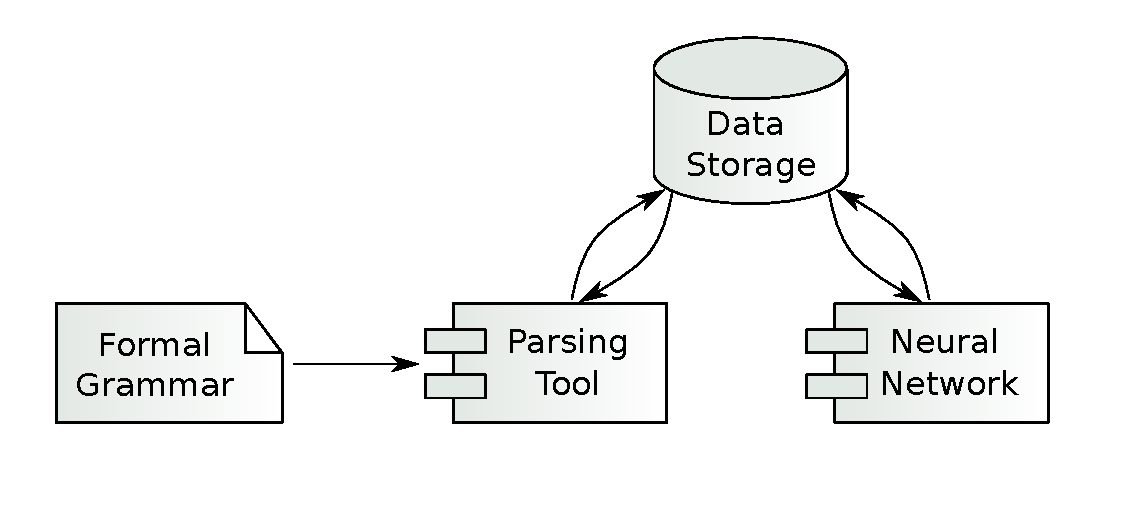
\includegraphics[width=12.0cm]{pics/diagram.pdf}
\caption{Архитектурные компоненты предложенного подхода}
\label{diagram}
\end{center}
\end{figure} 

Одной из потенциальных областей применения такого подхода является биоинформатика, в частности, различные задачи анализа РНК, где в качестве символьных последовательностей можно рассмотреть нуклеотидные цепочки РНК различных организмов, а в качестве синтаксической структуры --- биологическую вторичную структуру молекулы РНК. В текущей работе исследуется возможность применения описанного выше подхода для решения задачи предсказания вторичной структуры РНК. Далее будет описана разработанная для этого архитектура решения, включающая в себя два основных шага: задание грамматики для поиска характерных элементов вторичной структуры, а затем -- проектирование и обучение нейронных сетей, генерирующих для последовательности РНК максимально близкую к реальной вторичную структуру на основе полученных с помощью парсера данных.

\subsection{Формальная грамматика}
Первичная структура молекулы РНК представляет собой цепочку из нуклеотидов четырех типов (аденин, цитозин, гуанин и урацил), что в терминах синтаксического анализа есть последовательность символов алфавита \{A, C, G, U\}; вторичная же структура образовывается вследствие того, что некоторые участки первичной соединяются между собой, формируя рекурсивную композицию из шпилек разного размера и степени вложенности. Обобщенный вид таких шпилек может быть формализован средствами достаточно простой контекстно-свободной грамматики, каковой является используемая в данной работе грамматика $G_0$ (рис.~\ref{gram}). Грамматика учитывает только Уотсон-Криковские правила формирования нуклеотидных пар $A-U$, $C-G$ (строка \textbf{5}) и описывает рекурсивные композиции шпилек высоты от трех и более (строки \textbf{7-12}). Размер петли внутри шпильки лежит в пределах от одного до двадцати нуклеотидов, и такую же длину имеют последовательности, расположенные между любыми двумя шпильками (строка \textbf{2}). Эти числа были выбраны путем балансирования между следующими двумя соображениями: соответствие эмпирическим наблюдениям биологических данных и адекватность напрямую зависящих от длины и сложности грамматики временных затрат на работу парсера. По тем же причинам в $G_0$ не были включены неканонические нуклеотидные связи, которые могут встречаться в реальной вторичной структуре РНК --- для того, чтобы учесть все возможные пары нуклеотидов, придется ввести большое количество правил, имеющих вероятностную природу. Кроме того, средствами контекстно-свободных грамматик невыразимы псевдоузлы, однако псевдоузел есть комбинация из двух шпилек, следовательно, $G_0$, не описывая псевдоузел как единое целое, позволяет, тем не менее, выделить из входной последовательности обе составляющие его подстроки. Здесь становится понятным основное отличие нашего подхода от классического использования формальных грамматик в данной области~\cite{knudsen1999rna,dowell2004evaluation,rivas2000language} --- мы не пытаемся ни смоделировать вторичную структуру целиком, ни описать все возможные закономерности ее образования, но разбиваем ее на простые составные части, синтезировать из которых более сложные объекты предлагается уже с помощью нейронных сетей, что кратно уменьшает интеллектуальные и вычислительные затраты на синтаксический анализ.

\begin{figure}[h]
\begin{Verbatim}[numbers=left,xleftmargin=5mm]
s1: stem<s0>
any_str : any_smb*[1..20]
s0: any_str | any_str stem<s0> s0
any_smb: A | U | C | G
stem1<s>: A s U | G s C | U s A | C s G 
stem2<s>: stem1< stem1<s> >
stem<s>:  
      A stem<s> U 
    | U stem<s> A 
    | C stem<s> G 
    | G stem<s> C 
    | stem1< stem2<s> >  
\end{Verbatim}
\caption{Контекстно-свободная грамматика $G_0$ для описания шпилек вторичной структуры РНК}
\label{gram}
\end{figure}

Рассмотрим теперь формальный вид и практический смысл результата работы синтаксического анализатора для вышеописанной грамматики и последовательности РНК некоторого организма. Синтаксический анализ в данном случае используется для поиска всех подстрок входной строки, выводимых из стартового нетерминала $s1$ грамматики $G_0$, иными словами, для поиска тех участков этой строки, которые, в терминах $G_0$, могут свернуться в шпильки при формировании вторичной структуры. Формально, для входной строки $w$ парсер заполнит верхнетреугольную булеву матрицу --- матрицу разбора $M_P$, где $M_P[i,j]=1 \iff$ подстрока $w[i..j]$ выводится в $G_0$. Так как интересующие нас шпильки должны иметь высоту от трех, каждой шпильке высоты $n$ в матрице разбора будет соответствовать цепочка из $n - 2$ единиц. На рис.~\ref{mtrx} представлен результат работы парсера для изображенного на рис.~\ref{rna_a} случая последовательности, сворачивающейся в шпильку высоты четыре. Каждой нуклеотидной связи, образующей шпильку высоты от трех (сплошные линии голубого цвета), соответствует единица в ячейке матрицы разбора, при этом очевидно, что шпилька высоты три инкапсулирует в себе шпильки высоты два и один, обозначенные на рисунке пунктирными линиями. Помимо уже знакомой нам шпильки с рис.~\ref{rna_a}, в данной строке парсер обнаружил еще одну выводимую в грамматике подстроку (единица в позиции $[0,11]$): таким образом, для рассматриваемой цепочки существует два теоретически возможных варианта свертки, из которых реализованным на практике оказался только один.

\begin{figure}[h]
\begin{center}
\centering
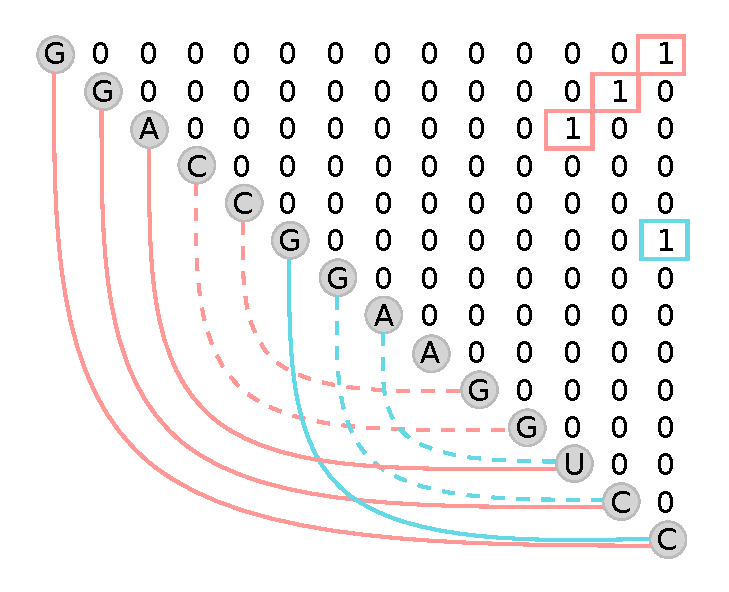
\includegraphics[width=10.0cm]{pics/matrix.pdf}
\caption{Матрица разбора для последовательности РНК}
\label{mtrx}
\end{center}
\end{figure} 
\vspace{3mm}

Остановимся в контексте предложенного подхода на проблеме обработки псевдоузлов, которые, как уже упоминалось ранее, не выводимы в используемой грамматике $G_0$. На рис.~\ref{pk_a} представлен пример последовательности, сворачивающейся в псевдоузел, а на рис.~\ref{pk_b} --- соответствующая данной последовательности матрица разбора. Рассматриваемый псевдоузел состоит из двух взаимопересекающихся шпилек высоты три и четыре, каждая из которых по отдельности выводима в $G_0$ и, следовательно, будет отражена в матрице разбора одной и двумя единицами соответственно. Несмотря на то, что на этапе синтаксического анализа еще не известно, образуют ли эти две найденные шпильки псевдоузел или же являются просто двумя теоретически возможными вариантами свертки цепочки, для нашего подхода предсказание псевдоузлов не становится ни сложностью, ни ограничением, так как матрицы разбора содержат всю необходимую о них информацию, которая должна быть более четко интерпретирована уже на этапе анализа данных нейронными сетями.

\captionsetup[subfigure]{justification=centering}
\begin{figure}[h]
\centering
\begin{subfigure}{.3\textwidth}
  \centering
  \fbox{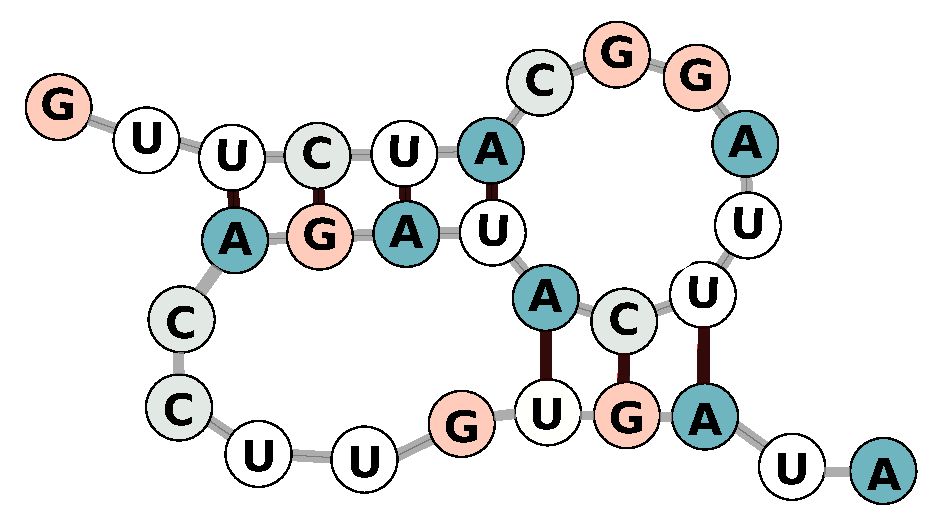
\includegraphics[width=.9\linewidth]{pics/pk.pdf}}
  \caption{Псевдоузел}
  \label{pk_a}
\end{subfigure}%
\begin{subfigure}{.7\textwidth}
  \centering
  \fbox{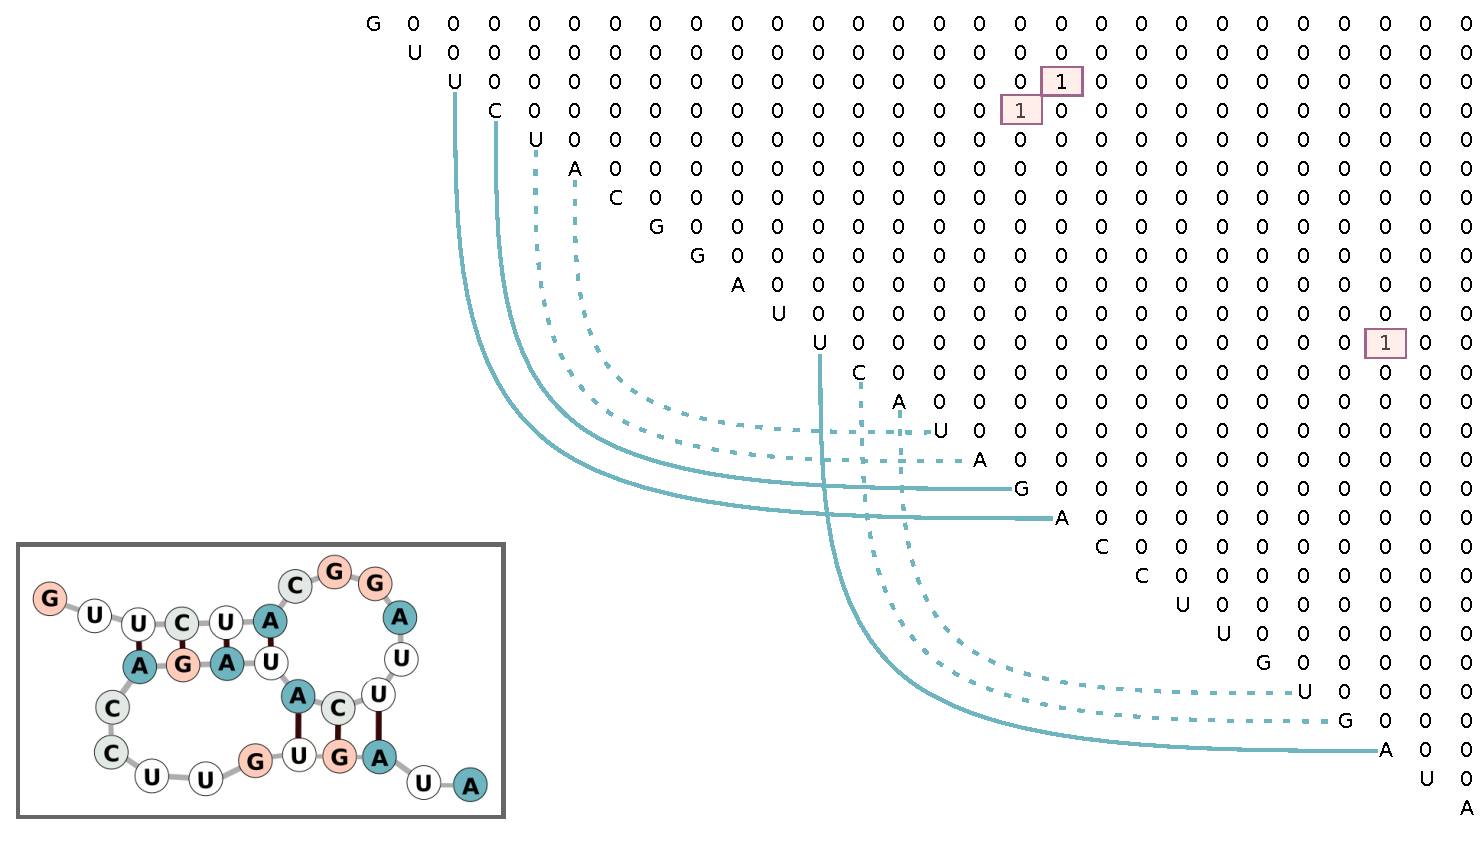
\includegraphics[width=.9\linewidth]{pics/matrix2.pdf}}
  \caption{Матрица разбора для последовательности с псевдоузлом}
  \label{pk_b}
\end{subfigure}
\caption{Обработка псевдоузлов в рамках предложенного подхода}
\label{pk}
\end{figure}

Таким образом, матрицы разбора хранят информацию о всех возможных расположениях шпилек вторичной структуры во входных последовательностях, однако на данный момент это только теоретические, искусственные объекты, для соотнесения которых с реальными биологическими данными требуется последующая обработка, и об этом будет подробно рассказано в следующем разделе.

\subsection{Нейронная сеть}
На данном этапе поставленная задача конкретизируется до следующей --- разработать нейронную сеть, которая принимает на вход матрицы, полученные синтаксическим анализатором по грамматике $G_0$ для некоторого набора последовательностей РНК, и, обучаясь на вторичных структурах, предоставленных в качестве эталонных для рассматриваемых последовательностей, оптимизирует параметры для преобразования матриц разбора в корректные вторичные структуры. Данный раздел посвящен описанию всех тонкостей этого процесса. 

\subsubsection{Подготовка данных} 
Входные данные для нейросети (матрицы разбора) были описаны в прошлом разделе, и теперь необходимо определить источник и формат эталонных данных. Существуют специализированные биологические базы данных, в которых размещены цепочки РНК различных организмов вместе с их извлеченными из природного материала или же полученными надежными методами вторичными структурами. Такие данные оптимальны для валидации, а, следовательно, и для обучения предсказывающих вторичную структуру алгоритмов. 

Как правило, в базах данных вторичные структуры РНК хранятся в скобочной (dot-bracket) нотации, из которой легко получить еще один классический формат  представления вторичной структуры --- так называемую матрицу контактов (contact map). Матрица контактов описывает наличие или отсутствие связи между каждыми двумя нуклеотидами последовательности: формально, для строки $w$ это верхнетреугольная булева матрица $M_C$, где $M_C[i,j]=1 \iff w[i]$ и $w[j]$ образуют пару во вторичной структуре. Как было описано в прошлом разделе, результат работы парсера на входной строке $w$ --- верхнетреугольная булева матрица $M_P$, где $M_P[i,j]=1 \iff w[i..j]$ свернется в шпильку по правилам грамматики. Нетрудно проверить, что наличие контакта между нуклеотидами $w[i]$ и $w[j]$ эквивалентно тому факту, что последовательность $w[i..j]$ является шпилькой, поэтому, несмотря на то, что наше определение вторичной структуры как композиции вложенных шпилек не относится к общеупотребимым, матрицу разбора можно также описать как матрицу контактов, формируемых только выразимыми в грамматике элементами. Таким образом, использование матричного представления вторичной структуры при подготовке эталонных данных для нейронной сети представляется самым удобным в свете специфики используемых в качестве входных данных матриц разбора. 

Для наглядности и удобства применения нейронных сетей мы предлагаем смотреть на матрицу контактов и матрицу разбора как на изображения: пикселями белого цвета обозначим позиции в матрицах с единицами, черного --- с нулями. Матрицы разбора содержат $n - 2$ единицы для каждой шпильки высоты $n>3$, следовательно, в качестве предобработки перед обучением нейросети для каждой единицы в матрице разбора следует добавить еще две единицы в направлении главной диагонали. Кроме того, сама нуклеотидная последовательность РНК может содержать некоторую важную информацию, поэтому предлагается закодировать ее на главной диагонали изображений равноотстающими друг от друга серыми пикселями. 

На рисунке~\ref{struc} продемонстрировано, как для одной и той же последовательности РНК будут выглядеть входной и эталонный образцы для нейронной сети, а также показана визуализация соответствующей вторичной структуры. Контакты, относящиеся к трем присутствующим в рассматриваемой цепочке шпилькам, на всех изображениях выделены голубым, сиреневым и розовым цветами. Данный рисунок является наглядным примером того, что далеко не все найденные парсером шпильки будут представлены в реальной вторичной структуре (белые пиксели изображения~\ref{struc_c}). Кроме того, видно, что в сгенерированной синтаксическим анализатором матрице отсутствует несколько эталонных контактов: в данном случае это произошло из-за того, что они были образованы непредусмотренными грамматикой неканоническими нуклеотидными парами. 

\captionsetup[subfigure]{justification=centering}
\begin{figure}[h]
\centering
\begin{subfigure}{.3\textwidth}
  \centering
  \fbox{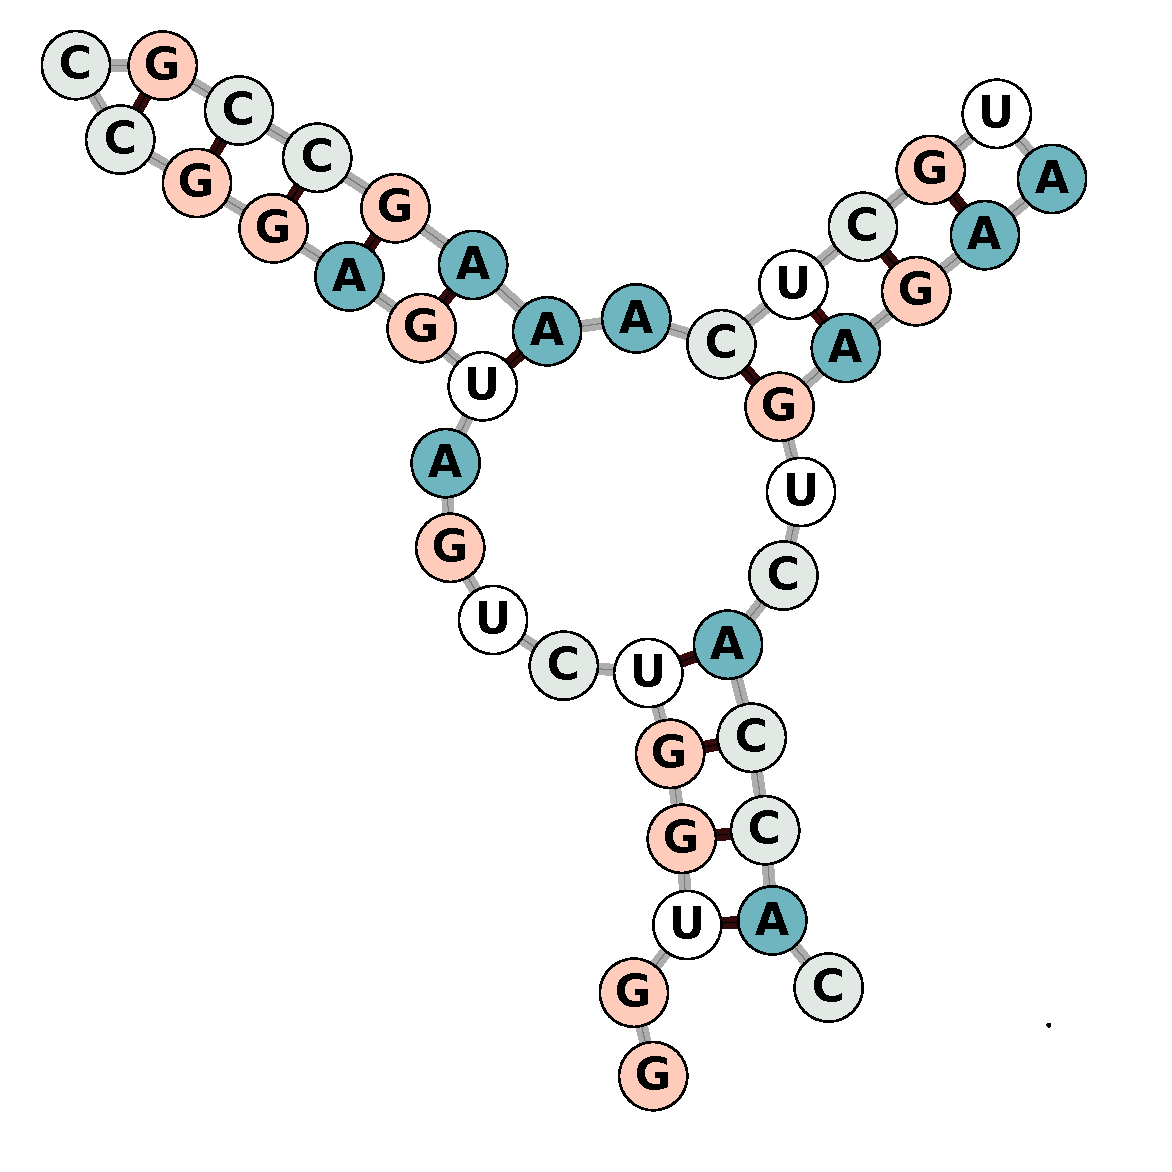
\includegraphics[width=.9\linewidth]{pics/struct.pdf}}
  \caption{Визуализация вторичной структуры}
  \label{struc_a}
\end{subfigure}%
\begin{subfigure}{.3\textwidth}
  \centering
  \fbox{
\includegraphics[width=.9\linewidth]{pics/out.png}}
  \caption{Эталонный  образец \\ для нейросети}
  \label{struc_b}
\end{subfigure}
\begin{subfigure}{.3\textwidth}
  \centering
  \fbox{
\includegraphics[width=.9\linewidth]{pics/in.png}}
  \caption{Входной образец \\ для нейросети}
  \label{struc_c}
\end{subfigure}
\caption{Примеры представления вторичной структуры}
\label{struc}
\end{figure}

Таким образом, в рамках данного исследования перед нейронной сетью стоит задача отфильтровать и дополнить матрицу разбора, сгенерировав корректную матрицу контактов, соответствующую максимально близкой к эталонной вторичной структуре.

\subsubsection{Параллельная остаточная архитектура}
Рассмотрим общую модель нейронной сети, разработанной в рамках данной работы. Входными и выходными данными являются изображения, и для решения поставленной задачи необходимо найти достаточно сложные закономерности между элементами данных, находящимися на большом расстоянии друг от друга, поэтому была использована глубокая сверточная сеть. Для оптимизации процесса обучения и повышения скорости сходимости была применена технология остаточных нейронных сетей. В процессе экспериментальных исследований нами было выявлено, что точность результатов значительно повышает использование $n$ остаточных сетей с одинаковой архитектурой, которые обучаются параллельно на одних и тех же данных, находя в них, по всей видимости, немного разные паттерны, а затем соединяются слоем, подсчитывающим линейную комбинацию их $n$ выходов и передающим ее уже общему остаточному блоку, завершающему обработку данных. Такая новая параллельная архитектура представлена на рис.~\ref{nn}; там же показано, как выглядит типичный остаточный блок (residual unit) нейронной сети, состоящий из пяти сверточных слоев с постепенно убывающими количеством фильтров и размером ядра свертки. В данной работе была использована модель, состоящая из четырех остаточных сетей с пятью одинаковыми блоками в каждой.

\begin{figure}[h]
\begin{center}
\centering
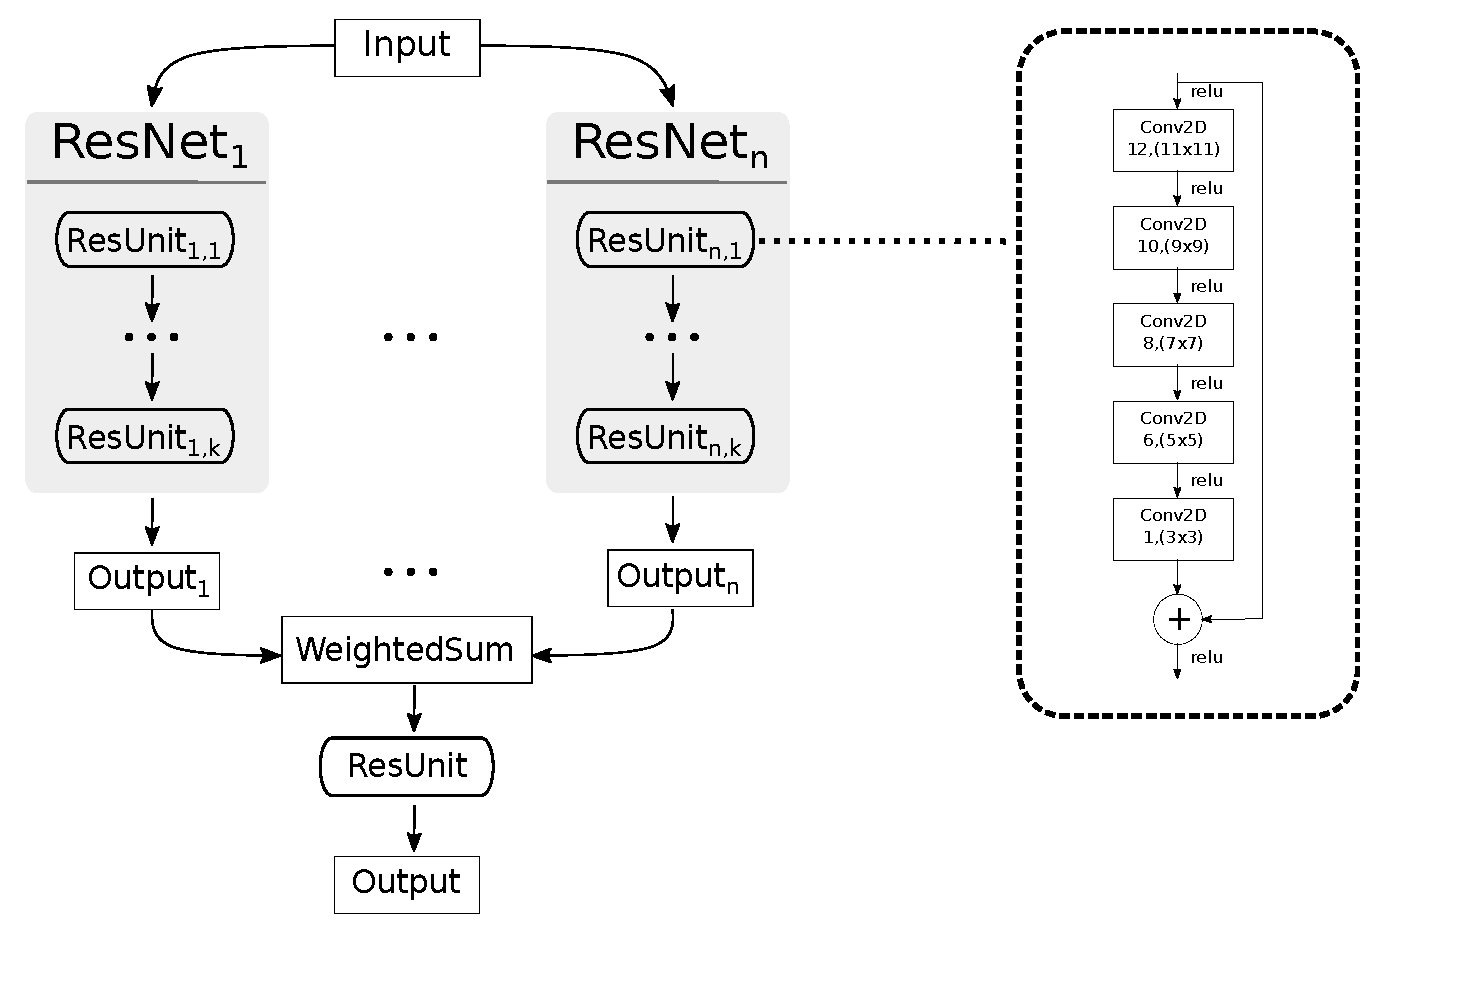
\includegraphics[width=15cm]{pics/nn.pdf}
\caption{Параллельная остаточная нейронная сеть}
\label{nn}
\end{center}
\end{figure} 
\begin{frame}[fragile]
	\transwipe[direction=90]
	\frametitle{\faCode\ Добавление новых возможностей}
	
	\begin{columns}
        \begin{column}{0.5\textwidth}
            \begin{figure}[t]{\textwidth}
				\centering
				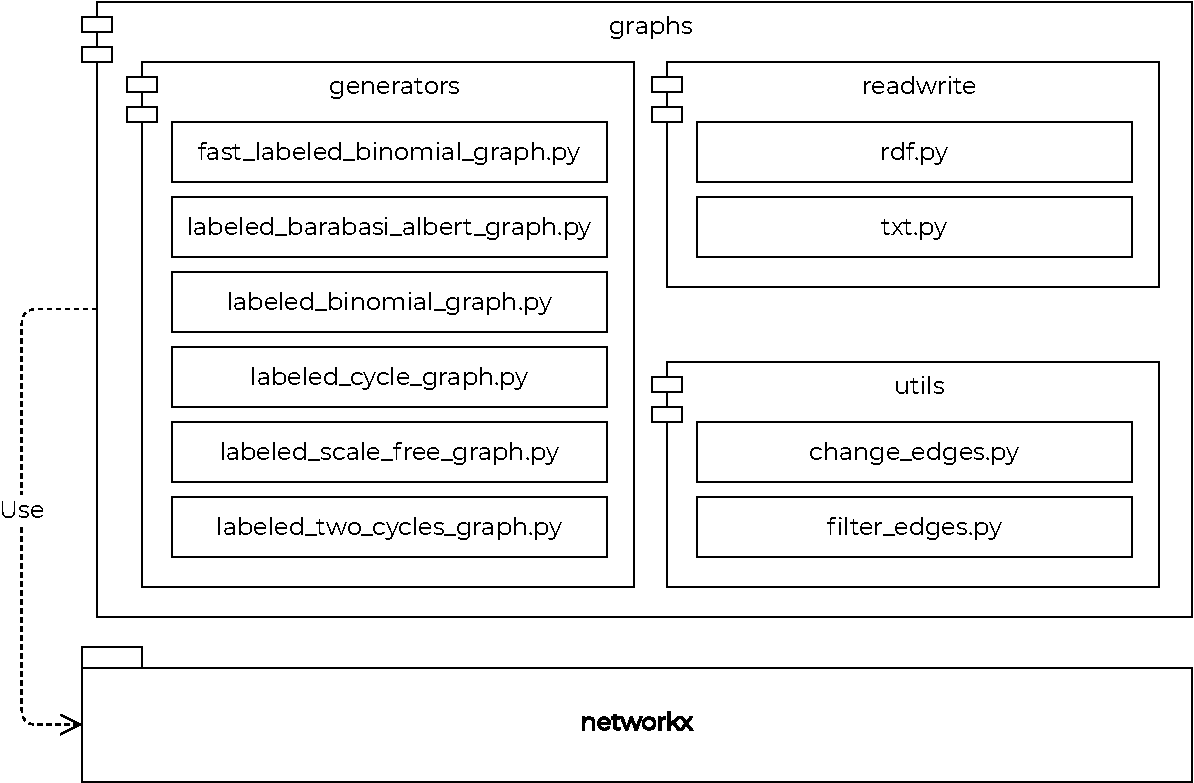
\includegraphics[width=0.96\textwidth]{img/graphs.pdf}
				\caption*{Рис. 5. Модуль работы с графами} \label{fig:graphs}
			\end{figure}
        \end{column}

        \begin{column}{0.5\textwidth}
            \begin{figure}[t]{\textwidth}
				\centering
				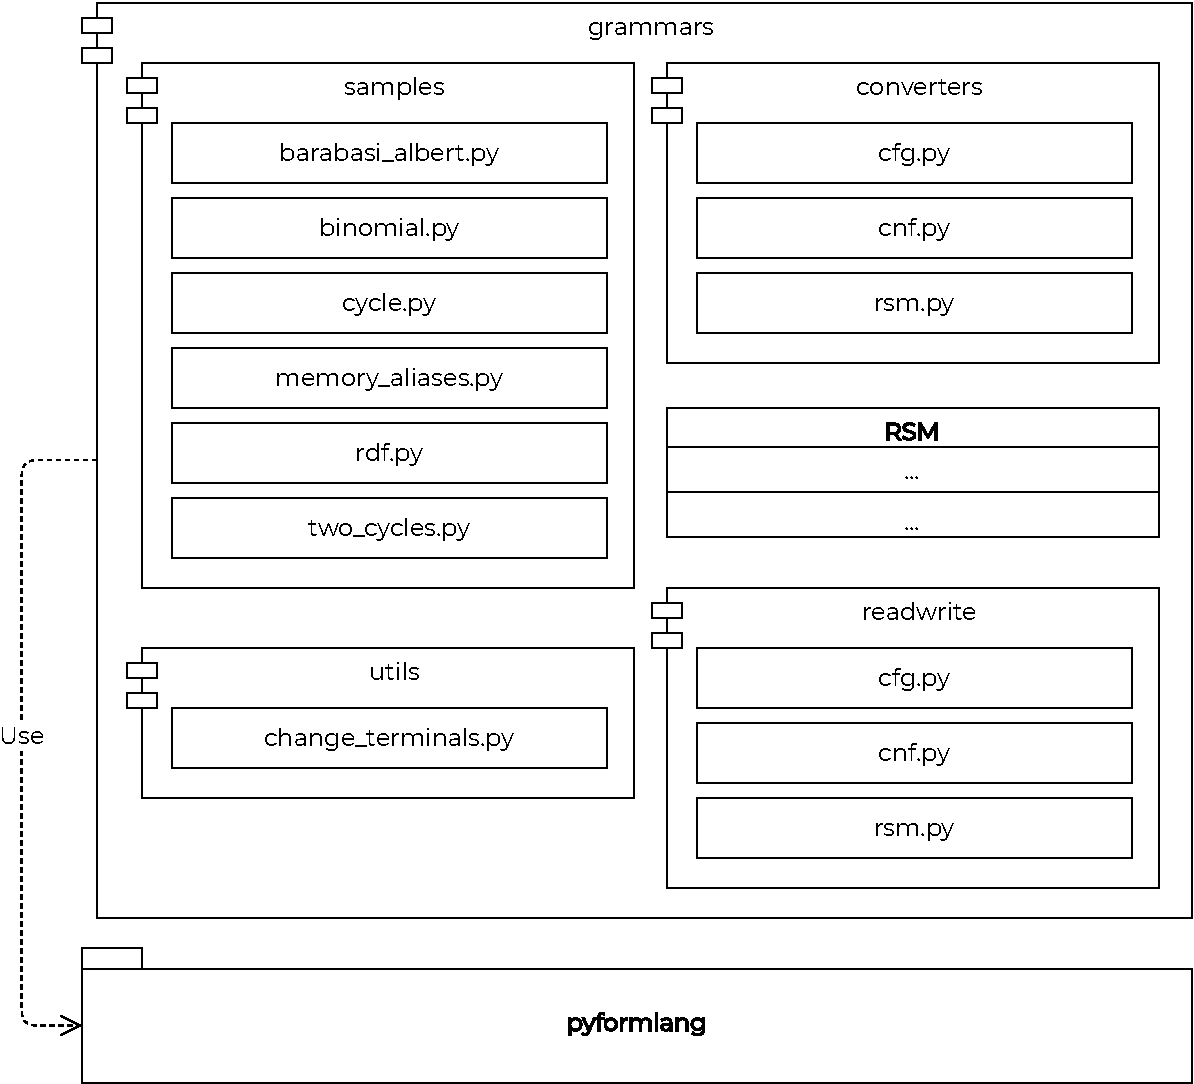
\includegraphics[width=0.96\textwidth]{img/grammars.pdf}
				\caption*{Рис. 6. Модуль работы с грамматиками} \label{fig:grammars}
			\end{figure}
        \end{column}
    \end{columns}
\end{frame}

\begin{frame}[fragile]
	\transwipe[direction=90]
	\frametitle{\faCloudUpload\ Публикация пакета}
	
	\begin{columns}
        \begin{column}{0.75\textwidth}
            \begin{figure}[h]{\textwidth}
        		\centering
        		\tcbox[color=black,boxsep=0mm, boxrule=0.3mm,colback=white]{
        		    \includegraphics[height=0.6\textheight]{img/website_new.pdf}
        		}
        		\caption*{Рис. 8. Веб-сайт проекта} \label{fig:website}
        	\end{figure}
        \end{column}

        \begin{column}{0.25\textwidth}
            \begin{itemize} 
        	    \item[\bullet] Информация о наборе данных
        	    \item[\bullet] Руководство по установке
        	    \item[\bullet] Обучающее руководство
        	    \item[\bullet] Документация
            \end{itemize}
        \end{column}
    \end{columns}
\end{frame}

\section{Модернизация набора данных \textsc{CFPQ\_Data}}

В результате обзора предметной области в проект \textsc{CFPQ\_Data} были внесены следующие изменения.
\begin{itemize}
    \item Было изменено стандартное представление графов и грамматик.
    \item Обновлено и расширено множество функций, предоставляемых проектом.
    \item Доступ к набору данных изменен с интерфейса командной строки на Python пакет, опубликованный в PYPI\footnote{Python пакет <<\textsc{CFPQ\_Data}>>: \url{https://pypi.org/project/cfpq-data/}, дата последнего доступа --- 04.06.2021}.
    \item Добавлено и автоматизировано интеграционное тестирование.
    \item Обновлен веб-сайт и автоматизирована его публикация.
\end{itemize}

\subsection{Представление данных}

Представление графа в виде множества записей вида <<объект, предикат, субъект>> хотя и идеально соответствует структуре помеченного графа и позволяет компактным образом хранить граф, но не подходит для исследования и манипулирования графами.
Именно поэтому в качестве стандартного представления помеченного графа выбран класс <<MultiDiGraph>> из проекта <<networkx>>\footnote{GitHub репозиторий <<networkx>>: \url{https://github.com/networkx/networkx}, дата последнего доступа --- 04.06.2021}, который является одним из наиболее известных проектов для работы с графами, хорошо задокументирован и имеет внушительное сообщество.
Такое архитектурное решение позволяет применять к графам, имеющимся в \textsc{CFPQ\_Data}, весь богатый арсенал функций из проекта <<networkx>>, что несомненно упрощает их исследование и манипулирование ими.

По тем же причинам, в качестве стандартного представления кон\-текстно-свобод\-ной грамматики выбран класс <<CFG>> из проекта <<py\-form\-lang>>\footnote{GitHub репозиторий <<py\-form\-lang>>: \url{https://github.com/Aunsiels/pyformlang}, дата последнего доступа --- 04.06.2021}, который является одним из наиболее известных проектов для работы с формальными языками и, в том числе, с контекстно-свободными грамматиками.
Кроме того, было реализовано представление контекстно-свободной грамматики с помощью рекурсивного автомата~\cite{RSM}.

\subsection{Архитектура}

Все предоставляемые для работы с графами и грамматиками функции выделены в один пакет <<\textsc{CFPQ\_Data}>>.

\begin{figure}[h]
    \centering
    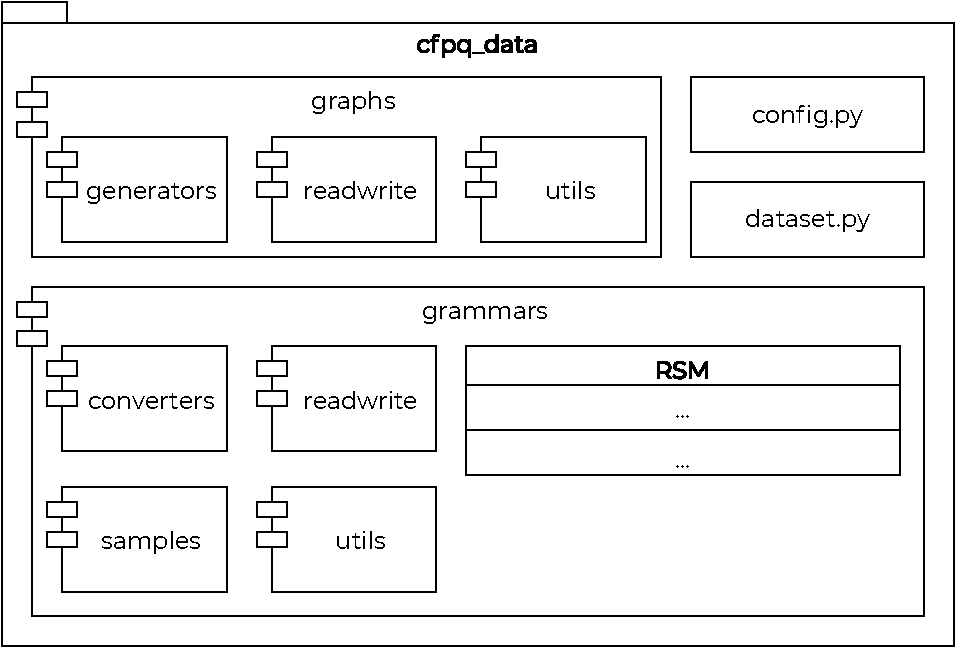
\includegraphics[width=\textwidth]{img/architecture_new.pdf}
    \caption{Новая архитектура \textsc{CFPQ\_Data}}
\end{figure}

Функции для манипулирования графами собраны в модуле <<graphs>>, который состоит из трех подмодулей.
\begin{itemize}
    \item В подмодуле <<generators>> реализованы функции генерации синтетических графов.
    \item В подмодуле <<readwrite>> реализованы функции чтения и записи графов, представленных в формате RDF и в формате троек <<вершина, метка ребра, вершина>>.
    \item В подмодуле <<utils>> реализованы функции для трансформации графов.
\end{itemize}

Функции для манипулирования грамматиками собраны в модуле <<grammars>>, который состоит из четырех подмодулей.
\begin{itemize}
    \item В подмодуле <<converters>> реализованы функции конвертации кон\-текстно-свобод\-ной грамматики между различными представлениями.
    \item В подмодуле <<readwrite>> реализованы функции чтения и записи кон\-текстно-свобод\-ной грамматики, представленной в различных форматах.
    \item В подмодуле <<samples>> реализованы примеры кон\-текстно-свобод\-ных запросов для соответствующих помеченных графов из <<graphs>>.
    \item В подмодуле <<utils>> реализованы функции для трансформации грамматик.
\end{itemize}

В файле <<dataset.py>> фиксируется информация о графах, сохраненных в \textsc{CFPQ\_Data}, соответствующая версии пакета, а в файле <<config.py>> фиксируется конфигурация доступа пакета к набору данных.

Также, с помощью GitHub Actions\footnote{GitHub Action интеграционного тестирования: \url{https://github.com/JetBrains-Research/CFPQ_Data/actions/workflows/tests.yml}, дата последнего доступа --- 04.06.2021} было реализовано интеграционное тестирование полученного пакета на юнит-тестах на различных операционных системах, с последующим сбором информации о покрытии кода.

\subsection{Документация}
Все предоставляемые пользователю функции были снабжены документацией, публикация которой добавлена в новой версии веб-сайта проекта.
Также на веб-сайт были добавлены следующие страницы.
\begin{itemize}
    \item Страница\footnote{<<Dataset>>: \url{https://jetbrains-research.github.io/CFPQ_Data/dataset/index.html}, дата последнего доступа --- 04.06.2021} с описанием графов из набора данных \textsc{CFPQ\_Data}.
    \item Страница\footnote{<<Install>>: \url{https://jetbrains-research.github.io/CFPQ_Data/install.html}, дата последнего доступа --- 04.06.2021} с руководством по установке пакета.
    \item Страница\footnote{<<Tutorial>>: \url{https://jetbrains-research.github.io/CFPQ_Data/tutorial.html}, дата последнего доступа --- 04.06.2021} с руководством помогающим начать пользоваться пакетом.
    \item Страница\footnote{<<Reference>>: \url{https://jetbrains-research.github.io/CFPQ_Data/reference/index.html}, дата последнего доступа --- 04.06.2021} с документацией всех функций, имеющихся в пакете.
    \item Страница\footnote{<<About>>: \url{https://jetbrains-research.github.io/CFPQ_Data/about.html}, дата последнего доступа --- 04.06.2021} с информацией о группе разработчиков проекта.
    \item Страница\footnote{<<License>>: \url{https://jetbrains-research.github.io/CFPQ_Data/license.html}, дата последнего доступа --- 04.06.2021} с лицензией проекта.
\end{itemize}

Также было сохранено индексирование проекта в Google Dataset Search и автоматизирована публикация сайта на GitHub Pages с помощью GitHub Actions\footnote{GitHub Action публикации веб-сайта: \url{https://github.com/JetBrains-Research/CFPQ_Data/actions/workflows/deploy_docs.yml}, дата последнего доступа --- 04.06.2021}.

\end{document}
